\section{\textsc{IntraCFG}: Intraprocedural Framework for Source-Level Control-Flow Analysis}%
\label{sec:IntraCFG}
The techniques of CFGs construction has seen significant advancements
in recent years, with various frameworks being proposed to aid in the construction
of precise intraprocedural CFGs~\cite{smits2020flowspec,10.1016/j.scico.2012.02.002}.
We contribute to the state-of-the-art by introducing \textsc{IntraCFG}, a declarative, RAG-based,
and language-independent framework for constructing precise intraprocedural CFGs.

Unlike most other frameworks, which build CFGs on the IR level,
e.g.,  bytecode, \textsc{IntraCFG}'s approach superimposes the CFGs
on the AST. This allows for a more accurate client analysis,
as the CFGs are constructed directly on the source code level, rather than an
intermediate representation. Additionally, this approach also enables the construction
of \textsc{AST-Unrestricted} CFGs, which are CFGs whose shape is not restricted to the AST structure.
\subsection{Overall Architecture}
The overall architecture of our proposed framework, \textsc{IntraCFG}, and its
ecosystem\todo{Not sure about the word ecosystem} is shown in Figure~\ref{fig:intraCFG}.
The framework provides the skeleton and default behaviour for construction of CFGs,
which can be instantiated for specific languages\footnote{\textbf{\texttt{IntraX}} in the diagram.}, e.g., Java or Teal.
\begin{figure}[H]
    \centering
    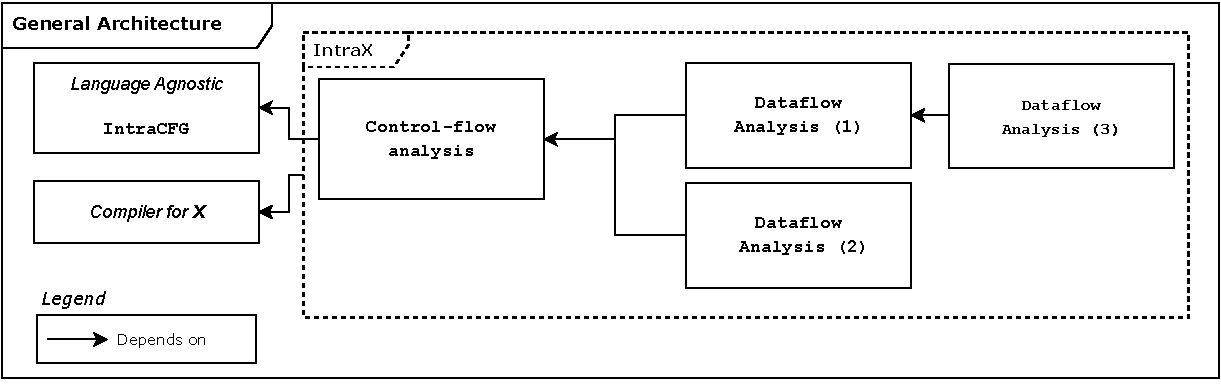
\includegraphics[width=1\textwidth]{kappa/img/architecture.pdf}
    \caption{\label{fig:intraCFG} Overall architecture of \textsc{IntraCFG} and its ecosystem.}
\end{figure}

The framework consists of several key components, including interfaces
(e.g., \textsc{CFGRoot}, \textsc{CFGSupport}, and \textsc{CFGNode}), attribute equations that define the
default behavior, and user APIs. The interfaces provide the structure for the
CFG and the attribute equations define the default behavior for the CFG
construction. Language specific AST nodes implement the different interfaces
according to the level of precision desired for the CFG.
The framework expose the CFG to the client analysis through APIs, that can be used
to query the CFG for information, such as the entry and exit nodes, or to traverse the CFG.
The language-independent nature of \textsc{IntraCFG} allows for easy integration
with various programming languages and enables the construction of precise CFGs
for those languages. The use of attribute equations and interfaces also allows
for a high degree of flexibility in the CFG construction process,
enabling the customization of the CFG to fit the specific needs of the
analysis being performed.

% Additionally, language-specific dataflow analysis, such as \texttt{NullPointerException} or
% \texttt{IndexOutOfBound} detection, can be built on top of the framework.





\subsection{\textsc{IntraCFG} for Java}
To demonstrate \textsc{IntraCFG} applicability, we developed
\textsc{IntraJ}, an instance of the framework for the Java programming language.
We built \textsc{IntraJ} as an extension of the \textsc{ExtendJ} extensible Java compiler~\cite{DBLP:conf/oopsla/EkmanH07}.
The complete architecture of \textsc{IntraJ} is shown in Figure~\ref{fig:intraJ}.
\begin{figure}[H]
    \centering
    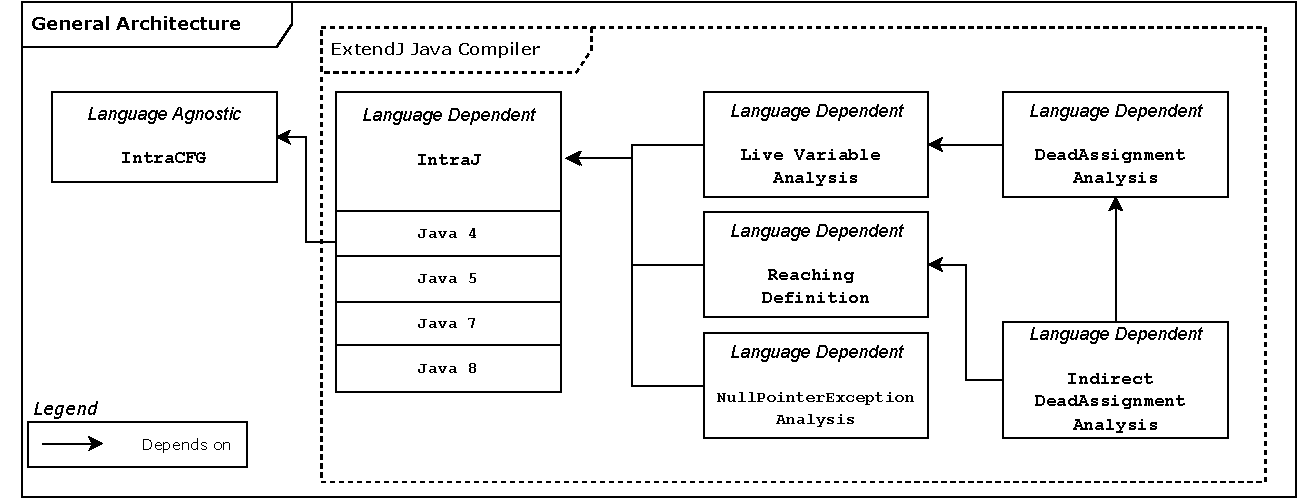
\includegraphics[scale=0.52]{kappa/img/architecturejava.pdf}
    \caption{\label{fig:intraJ} Overall architecture of \textsc{IntraCFG} instansiated for the Java language.}
\end{figure}

%Discussing modularity
We designed \textsc{IntraJ}, following a  modular approach, and we separately
instansiated the framework for different versions of Java such as Java 4,
Java 5, Java 7 and Java 8. Each version of Java is implemented as a separate
aspect of the compiler. This approach allows us and the users of \textsc{IntraJ}
to easily extend the framework to support new versions of Java.

% Discussing precision
The degree of precision in creating CFGs using \textsc{IntraCFG} can differ in order
to meet the requirements of a given application.
This flexibility allows us to optimize the efficiency of the analysis by selectively
excluding certain nodes from the CFG, such as \texttt{WhileStmt}, which do not
provide any information relevant to the analyses.
\begin{figure}[H]
	\centering
	\begin{tikzpicture}
		\node (a) at (3.5,0) {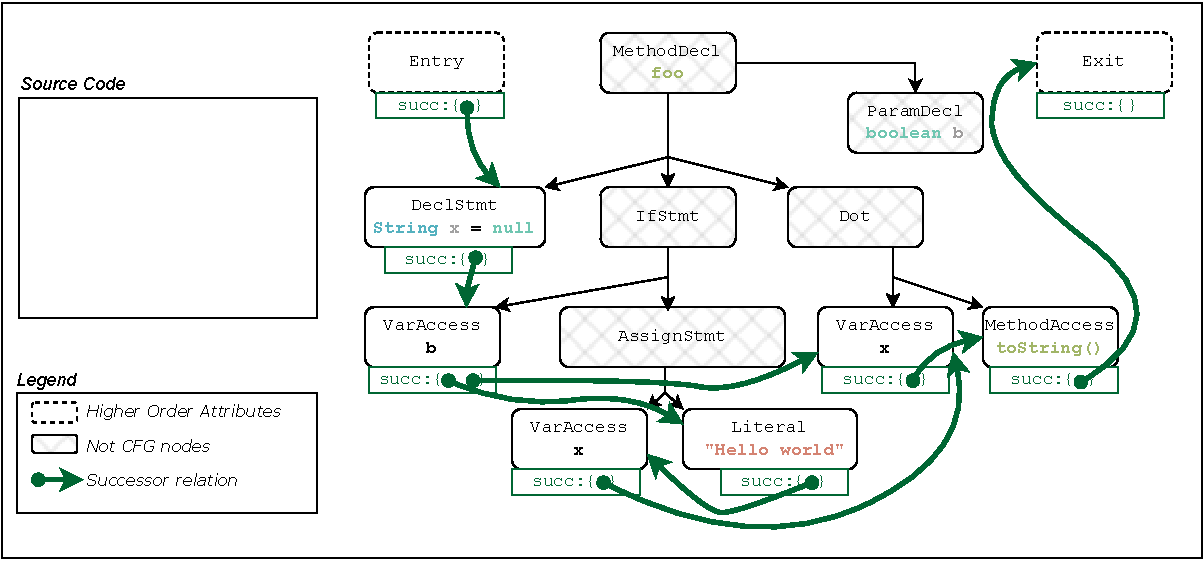
\includegraphics[scale=0.55]{kappa/img/exampleAST.pdf}};
		\node[scale=0.65] (b) at (-0.6,0.7) {
			\begin{lstlisting}[language=JastAdd]
void foo(boolean b){
  String x = null;
  if(b) {
    x = "Hello World";
  }
  x.toString();
}
			\end{lstlisting}
		};
	\end{tikzpicture}
	\caption{\label{fig:CFG} CFG of the \texttt{foo} Java method.}
\end{figure}

The example in Figure~\ref{fig:CFG} is a visual representation of the AST and CFG of the
\texttt{foo} Java method. The figure illustrates the ability of the framework to tailor the CFG
to the specific requirements of the analysis and eliminate unnecessary complexity for improved performance.
In this example, nodes like \texttt{IfStmt} or \texttt{Dot} are not included in the CFG,
resulting in a more concise but precise representation of the control flow of the program.
On the other hand, the precision of the CFGs can be improved by synthethizing new nodes and new subtrees.
For instance, we designed \textsc{IntraJ} to compute an exception-sensitive
control-flow analysis, i.e., new AST subtrees are synthesized for each possible exceptional path.
The resulting CFGs are more precise, but they are also more complex, resulting
in a higher memory consumption and a longer analysis time.



In \textsc{IntraJ}, we implemented five different dataflow analyses:
\begin{itemize}
  \item \emph{Live Variable Analysis}: This analysis computes the set of variables that are live at each program point.
  \item \emph{Reaching Definition}: computes the set of definitions that reach each program point.
  \item \emph{Null Pointer Analysis}: detects possible null pointer dereferences.
  \item \emph{Dead Assignment Analysis}: detects assignments to l-values that are never used from that point on.
  \item \emph{Indirect Dead Assignment Analysis}: detects assignments to l-values which uses always flow to a dead assignment.
\end{itemize}
All the analyses relie on the result of the control-flow analysis. To the analysis are exposed
the entry and exit nodes of the CFG, as well as the successor and predecessor
nodes of each node.
Each analysis is implemented as a separate aspect of the compiler. Nevertheless,
the result of some analyses is used as input for other analyses. For instance,
the result of Live Variable Analysis is used as input for the Dead Assignment Analysis.
Similarly, the result of Dead Assignment Analysis is used to compute Indirect Dead Assignment Analysis.

The implemented analyses are instances of the monotone frameworks (see Section~\ref{sec:monotoneframeworks}).
Each analysis defines its abstract domain, transfer function and \emph{in} and
\emph{out}\footnote{Sometimes can be named \emph{gen} and \emph{kill}.} attributes.
The language dependency of the dataflow analysis arises from the fact that the
transfer function, which defines the relationship between the \emph{in} and \emph{out},
is modeled as an attribute. This transfer function attribute is
define for each AST node in the CFG in order to capture the semantic of passing
through that node.



\subsection{\textsc{IntraCFG} for TEAL}
\begin{figure}[H]
    \centering
    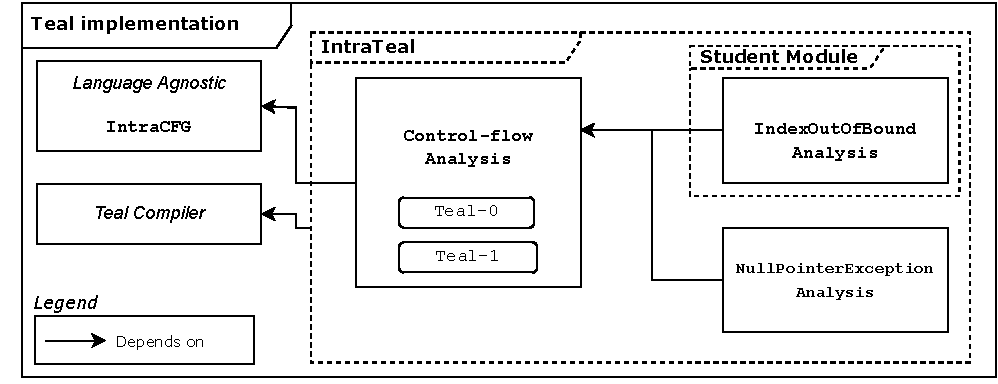
\includegraphics[scale=0.65]{kappa/img/architectureteal.pdf}
    \caption{\label{fig:IntraTeal} Overall architecture of \textsc{IntraCFG} instansiated for the Teal language.}
\end{figure}
As a further demonstration of the applicability of \textsc{IntraCFG},
we developed \textsc{IntraTeal}, an implementation of the framework for the Teal programming language.
The teal programming language is used for teaching purposes
and provides a simple and easy-to-learn syntax for students to understand the
concepts of static program analysis (see Section~\ref{sec:teal}).
As part of the course, the complete source code of \textsc{IntraTeal} was provided to students along with
instructions and guidelines for utilizing the API to implement their own analyses.
We also made available a reference implementation of the
\texttt{NullPointerException} analysis. We then asked students, as a way of
extending their understanding and skills, to implement an \texttt{IndexOutOfBound}
analysis on the interval abstract domain. This exercise provided the
students with an opportunity to apply the concepts they had learned in a practical
setting and gain a deeper understanding of dataflow analysis.

Another key aspect of both, \textsc{IntraTeal} and \textsc{IntraJ} implementations, is that they
construct enhanced control-sensitive CFGs. Control-sensitive CFGs
are a more precise representation of the control flow of a program, as they take
into account the specific control flow behavior of a program. This is achieved by
synthesizing two AST nodes, i.e., \texttt{ControlTrue} and \texttt{ControlFalse} for each
comparison operator, e.g.,  ``$\le$'', ``$==$'', ``$!=$'', inside a conditional statement.
These HOAs are used to represent the control flow of the program and the information that ca be inferred from
it. \\
%
\begin{minipage}{0.45\textwidth}
    \begin{lstlisting}[language=JastAdd,caption={Control-sensitivity to improve null pointer analysis.}, label={lst:control-null}]
if(x!=null){
  //x is not null here
}
    \end{lstlisting}
    \end{minipage}\hfill%
    \begin{minipage}{0.45\textwidth}
    \begin{lstlisting}[language=JastAdd,caption={Control-sensitivity to improve interval analysis.}, label={lst:control-interval}]
if(x > 4 and x <= 6){
    //x is [5,6] here
}
    \end{lstlisting}
\end{minipage}\\
The example in Listing~\ref{lst:control-null} shows how the \texttt{ControlTrue} and \texttt{ControlFalse}
HOAs are used to keep track of the information that the object \texttt{x} is not null
in the \emph{then} branch and null in the \emph{else} branch.
This information is used to improve the precision of the analysis and provide
more accurate results without affecting the performance of the analysis.

We also asked students to use the \texttt{ControlTrue} and \texttt{ControlFalse}
HOAs to improve the precision of the interval analysis. The example in
Listing~\ref{lst:control-interval} shows how the \texttt{ControlTrue} and \texttt{ControlFalse}
HOAs are used to keep track of the information that the object \texttt{x} is in the interval $[5,6]$.
\begin{figure}
	\centering
	\begin{tikzpicture}
		\node (a) at (0,0) {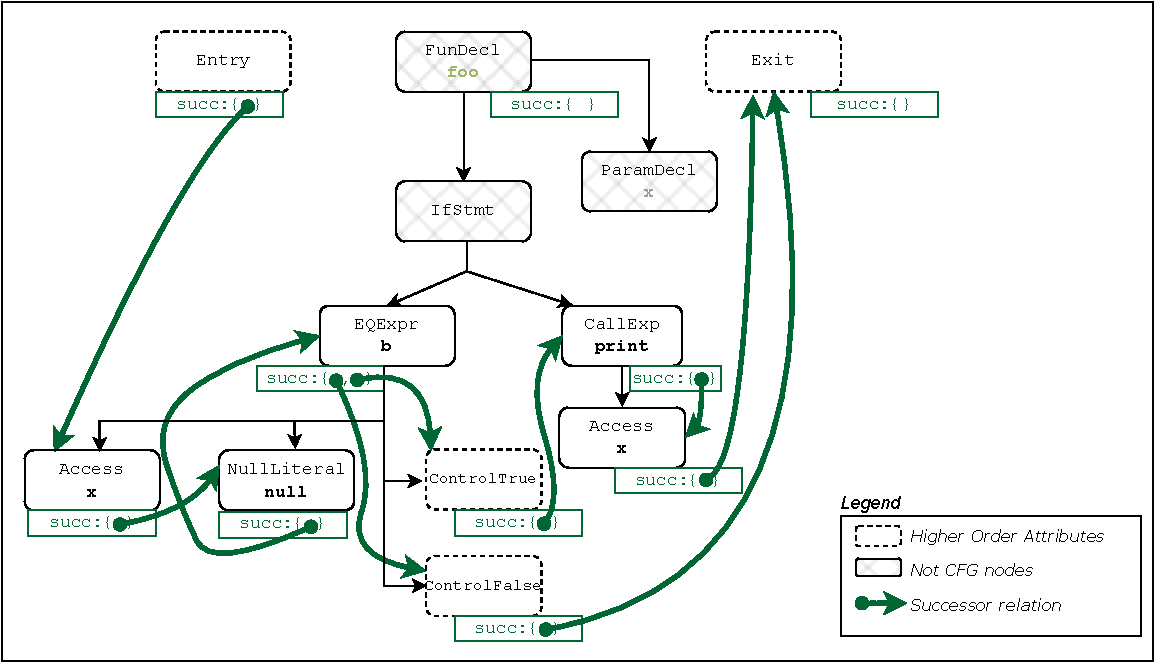
\includegraphics[scale=0.55]{kappa/img/TEALExample.pdf}};
		\node[scale=0.7] (b) at (3.5,0.45) {
			\begin{lstlisting}[language=JastAdd]
fun foo(x) = {
  if(x==null){
    print(x);
  }
}
			\end{lstlisting}
		};
	\end{tikzpicture}
	\caption{\label{fig:ExampleTEAL} Example of control-sensitivity in \textsc{IntraTeal}.}
\end{figure}
\begin{lstlisting}[language=JastAdd,label={lst:ControlTrueEq}, caption={Transfer function for \texttt{ControlTrue} HOA.}]
eq ControlTrue.nullnessTransfer(NullDomain lattice) {
  NullDomain result = new NullDomain(lattice);
  NullDomain assignment = getCond().getImplicitAssignment();
  return result.join(assignment);
}
\end{lstlisting}
The example presented in Figure~\ref{fig:ExampleTEAL} along with the code snippet
provided in Listing~\ref{lst:ControlTrueEq} illustrates how the precision of the
analysis is enhanced by considering implicit assignments~\cite{spa} in the control flow of
the program. Specifically, the transfer function for the \texttt{ControlTrue} HOA
takes into account that the object \texttt{x} is null when it is printed within
the \emph{then} branch of the \texttt{if} statement.


The task assigned to the students, which was an extension of the \texttt{NullPointerException}
analysis, was to implement an \texttt{IndexOutOfBound} analysis on the interval domain.
The interval domain, being an infinite domain, poses a significant challenge for
dataflow analysis due to the inherent nature of infinite domains. In particular,
the iterative nature of dataflow analysis algorithms, which rely on the computation
of a sequence of approximations, may not terminate when applied to an infinite domain.
This can result in an excessive consumption of computational resources and ultimately
lead to a failure of the analysis. Additionally, the use of infinite domains can also
lead to the presence of non-converging sequences, resulting in an analysis that does
not converge to a stable solution. The example in Figure~\ref{fig:nonConverging}
illustrates a non-converging program.
\begin{figure}
	\centering
	\begin{tikzpicture}
		\node (a) at (3.5,0) {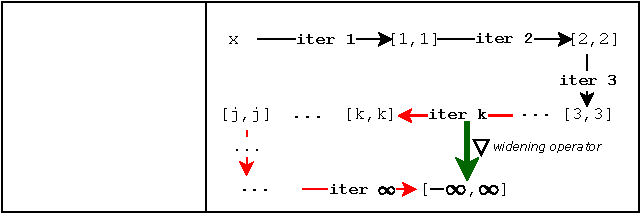
\includegraphics[scale=1]{kappa/img/non-convergin.pdf}};
		\node[scale=1] (b) at (-0.2,0) {
			\begin{lstlisting}[language=JastAdd]
fun foo(x) = {
  x := 0;
  while (true) {
    x = x + 1;
  }
}
			\end{lstlisting}
		};
	\end{tikzpicture}
	\caption{\label{fig:nonConverging} Trivial example of non-converging program.}
\end{figure}

To ensure the termination of the analysis, the students were required to
define their own widening operator~\cite{Bagnara2003Widening}.
However, \textsc{JastAdd} circular attributes, which are used to implement dataflow
analysis, do not natively support widening operators, as they are designed
to work only on finite lattices. To overcome this limitation, an ad-hoc solution
solution was implemented to trigger the widening operator after a certain
number of steps.

This experience highlights the need for native support for widening and narrowing
operators in \textsc{JastAdd}, to allow static analysis developers to effectively deal with
infinite lattices. In the future, we plan to investigate the implementation of this
feature in \textsc{JastAdd} to facilitate developers of static analysis tools.


\subsection{IDE Integration}
In this Section, we focus on the integration of \textsc{IntraJ} and \textsc{IntraTeal} with different
IDEs and developers tools. We first describe the integration of \textsc{IntraJ} with
IDEs that support the Language Server Protocol (LSP)~\cite{lsp}, such as
\textsc{Visual Studio Code}~\cite{vscode}, \textsc{Emacs}~cite{emacs}, and \textsc{Vim}\cite{vim}, using
the MagpieBridge~\cite{luo_et_al:LIPIcs:2019:10813} framework. We then describe the
integration of \textsc{IntraJ} and \textsc{IntraTeal} with \textsc{CodeProber}~\cite{risberg2022property},
a tool for visualising and exploring the results of compilers and static analysis tools.
This work, specifically the integration of the \textsc{IntraJ} static analyser with IDE through
the use of the MagpieBridge framework, is not described in the two attached papers.
However, it was developed as an application of the research and methods previously
described in these papers, and was carried out subsequently.

\subsubsection{LSP support via MagpieBridge: warnings, quick-fixes and bug explanations}
\begin{figure}
  \centering
  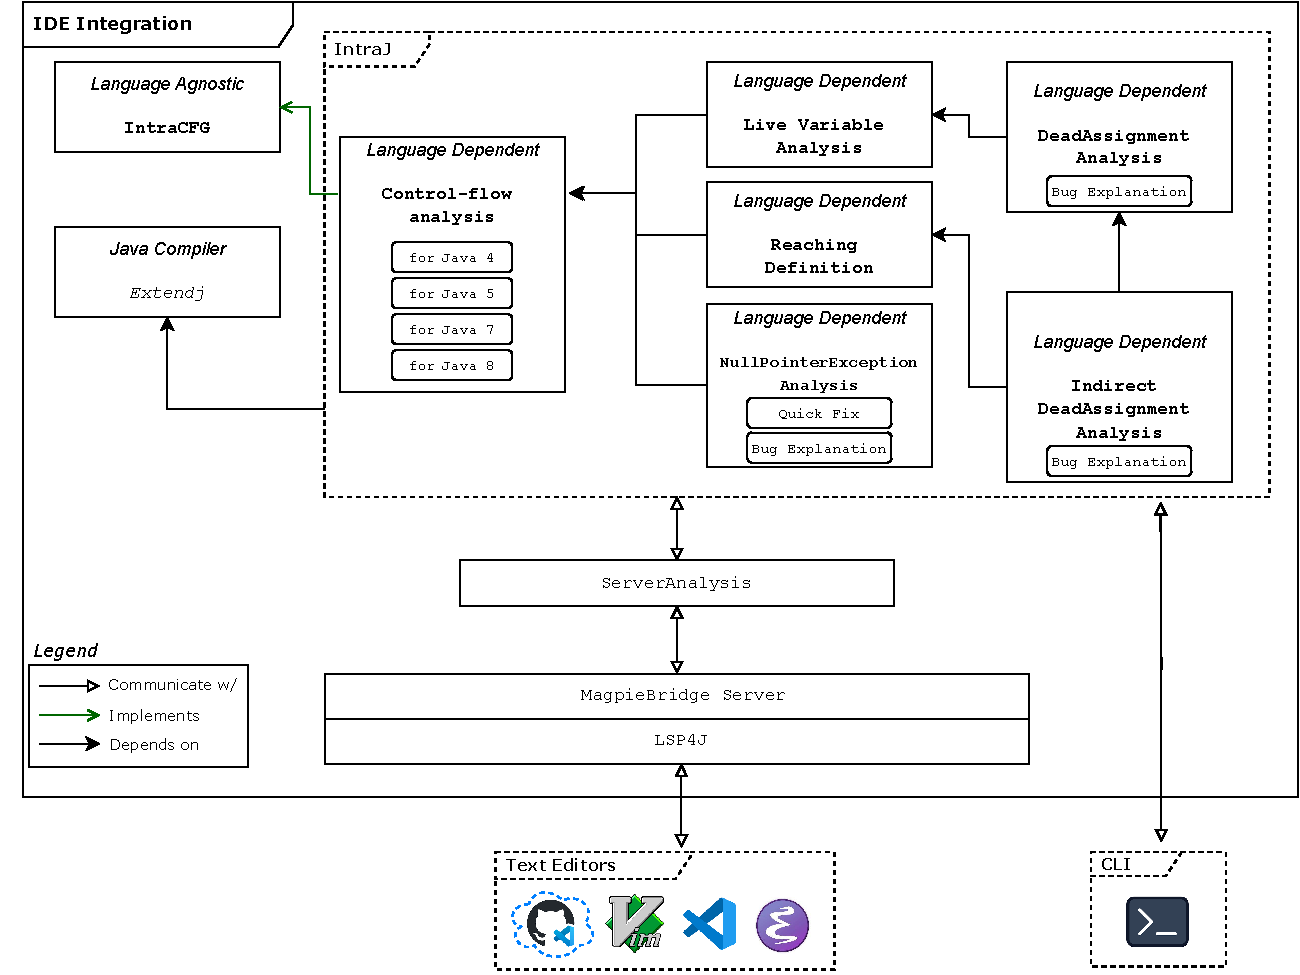
\includegraphics[width=0.92\textwidth]{kappa/img/IDEIntegration.pdf}
  \caption{\label{fig:IDEIntegration} Integration of \textsc{IntraJ} with IDEs through the use of the \textsc{MagpieBridge} framework.}
\end{figure}
Initially, \textsc{IntraJ} was developed as a command-line tool, which performance was competitive
compared to existing industrial tools. However, we recognized the potential
for further improvement, by exploting the on-demand evaluation feature of \textsc{JastAdd}.
On-demand evaluation enables the execution of dataflow analyses
on methods within open files, as opposed to the entire codebase. This approach
allows for user-centric, real-time feedback on complex bugs, providing developers
with instantaneous insights and facilitating efficient debugging and troubleshooting
processes.
To achieve this, we used the \textsc{MagpieBridge} framework, which facilitates the integration
of static analysers with IDEs that support the LSP. \textsc{MagpieBridge} provides an
abstraction layer between the IDE and the static analysis tool, simplifying the
integration process and allowing for the development of IDE plugins with minimal effort.
\textsc{MagpieBridge} provides an abstraction layer between the IDE and the static
analysis tool allowing the display of warnings, quick-fixes, and explanations
for bugs within the IDE, providing developers with a immediate and convenient way to
access and interact with analysis results, while also facilitating communication
between the static analysis tool and the IDE. Additionally, the framework allows
for the display of web pages within the IDE, providing developers with a new level
of support for visualization, customizable user interfaces, and a better way to
interact with analysis results.

Figure~\ref{fig:IDEIntegration} illustrates the integration of \textsc{IntraJ} with
different IDEs. \textsc{ServerAnalysis} is a component that we developed to handle the
communication between \textsc{IntraJ} and the \textsc{MagpieBridge} Server. It is responsible
for maintaining a record of the active analyses and forwarding events in the editor,
such as the save command or opening of a file, to the \textsc{IntraJ} tool.
The results of the analysis are then sent back to the \textsc{MagpieBridge}, which subsequently
forwards them to the editor, displaying warnings, quick-fixes, and explanations
to the developer.
\begin{figure}[ht]
  \centering
  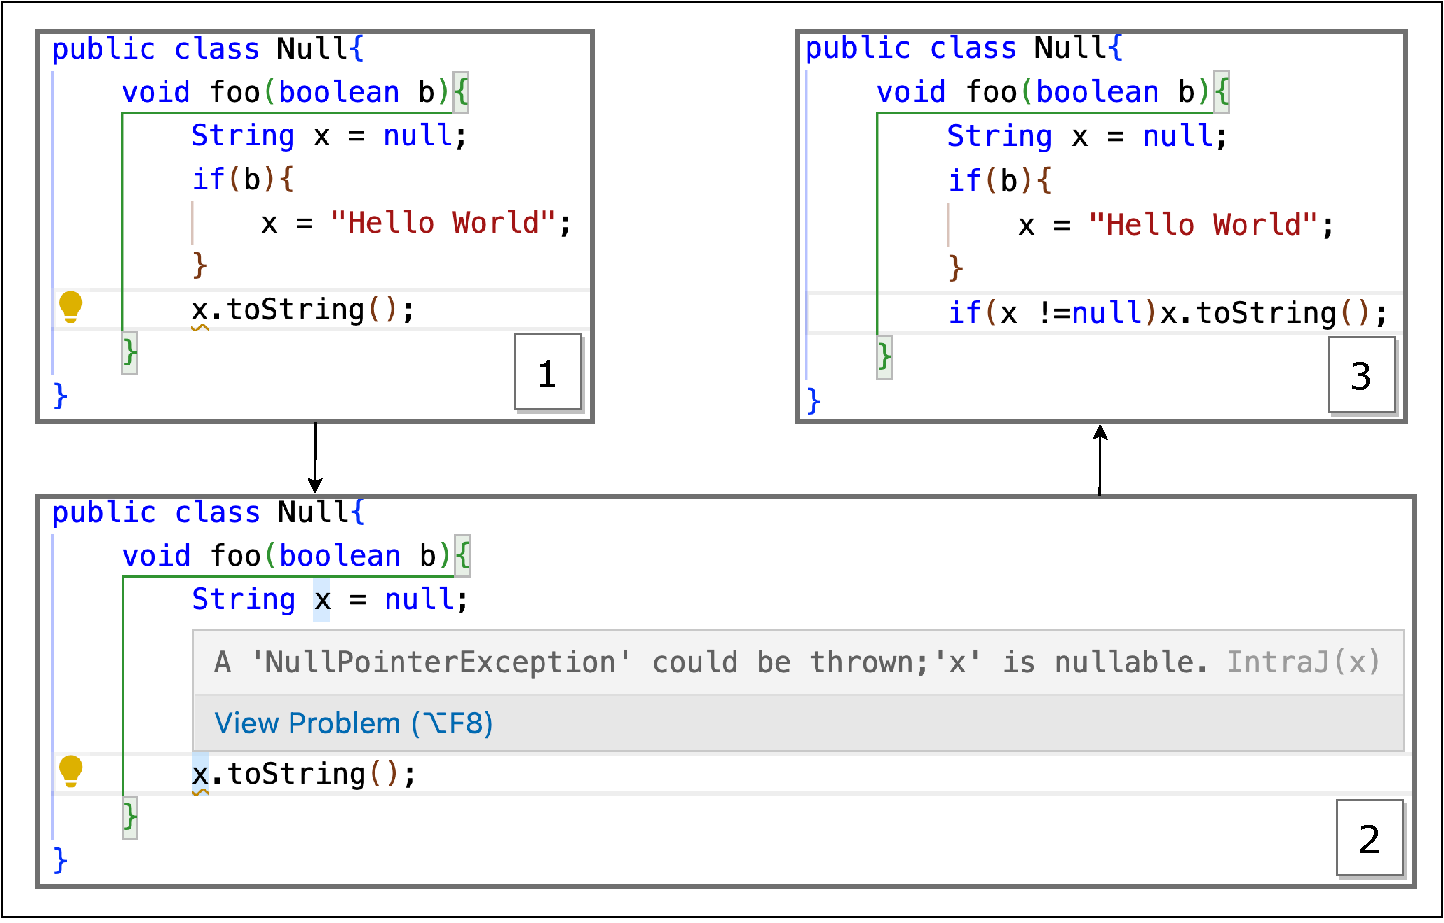
\includegraphics[width=0.92\textwidth]{kappa/img/IDEExample.pdf}
  \caption{\label{fig:IDEExample} Bug detection and quick-fix in \textsc{Visual Studio Code} using \textsc{IntraJ}.}
\end{figure}
To enable a better user experience, we extended the functionality of the existing analysis.
Specifically, we enhanced the \texttt{NullPointerException} analysis to not only detect issues
but also provide developers with quick fixes and explanations, allowing them to address
the problems more efficiently. Additionally, we enhanced the \texttt{(Indirect) Dead Assignment} analysis
to provide explanations, giving developers a deeper understanding of the issues detected.
Figure~\ref{fig:IDEExample} illustrates an example of interaction between \textsc{IntraJ} and
\textsc{Visual Studio Code}. More specifically, illustrates an instance of a \texttt{NullPointerException} 
detected by \textsc{IntraJ} and its representation within the IDE. 
The ``
\includegraphics[height=8pt]{kappa/img/bulb.png}''  icon indicates that an quick-fix is available,
which can be applied by clicking on the icon.

\subsubsection{Visualisation via \textsc{CodeProber}}
In this Section, we will give an overview of the integration of \textsc{IntraJ} and \textsc{IntraTeal}
with \textsc{CodeProber}, a tool for visualizing and 
exploring the results of compilers and static analysers. \textsc{CodeProber} 
allows developers to interact with the results of the analysis in a visual and intuitive 
manner. It enables real-time interaction with the AST node's attributes and the source code, 
enabling analyses developers to explore results and partial results, making 
debugging and troubleshooting more efficient with respect the traditional debugging
approaches. As a browser-based tool that is not restricted to the Language Server Protocol, 
\textsc{CodeProber} enables the visualisation of analysis results in different 
formats, including, but not limited to, graph representation and other visual forms, beyond
simply displaying warnings.
\begin{figure}[H]
  \centering
  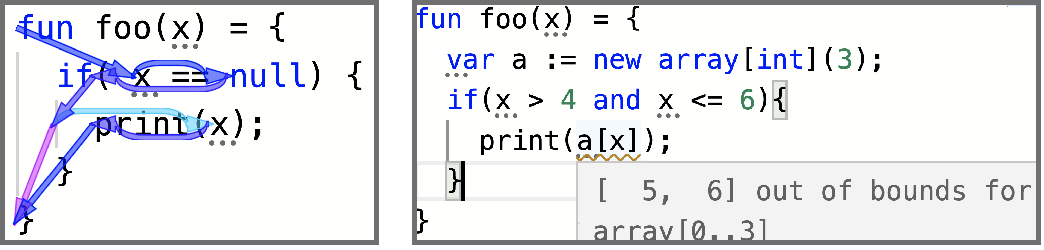
\includegraphics[width=0.92\textwidth]{kappa/img/CP.pdf}
  \caption{\label{fig:CodeProber} Interaction of \textsc{IntraTeal} in \textsc{CodeProber}.}
\end{figure}
The example in Figure~\ref{fig:CodeProber} shows the visual representation of the CFG on
top of the source code. The CFG is generated by \textsc{IntraTeal} and visualized by
\textsc{CodeProber}. The graph is rendered automatically at each change in the source code,
allowing developers to understand the flow of the program and all the possibile execution paths of the
analysis in real-time. 

We used the \textsc{IntraTeal} and \textsc{CodeProber} integration in the Program analysis
course. Students were able to understand the CFG and the flow of the program and 
were asked to identify \textsc{IndexOutOfBound} exceptions. Students were able to
observe their progress and the outcomes of thier analysis within a realistic IDE.



\section{\textsc{JFeature}: Java Feature Extractor}
\label{sec:JFeature}
\textsc{JFeature} is a static analysis tool for the Java programming language that extracts
syntactic and semantic features from Java programs. The tool is designed to assist
researcher and developers in selecting appropriate software corpora to better evaluate the robustness
and performance of software tools, such as static analyzers.
\textsc{JFeature} is implemented as an extension of the \textsc{ExtendJ} Java compiler. It is declarative
and extensible, allowing for the easy addition of new queries.

The need for \textsc{JFeature} arose during the evaluation of \textsc{IntraJ}.
While analyzing Java projects from the \textsc{DaCapo Benchmark suite}~\cite{DaCapo:paper} corpus to evaluate the precision
of \textsc{IntraJ} on Java 8 projects, it became apparent that there were no Java 8 projects
in the \textsc{Da Capo Benchmark suite}. Further investigation revealed that many
commonly used software corpora in the field of static analysis were lacking
representation of Java 8 projects.

To address this problem, we developed \textsc{JFeature}, a tool that extracts features from
Java programs categorised by the Java version they were introduced in.
The goal of \textsc{JFeature} is to provide insight and a comprehensive overview of 
the composition of a Java project or corpus, specifically in terms of the different 
Java features categorized by the Java version in use.
\textsc{JFeature} comes with twenty-six predefined queries and can be easily extended
with new ones. Since \textsc{JFeature} is built on top of the \textsc{ExtendJ} compiler, \textsc{JFeature} has access
to all the information computed by the compiler, allowing the definition of complex 
queries.
In Figure~\ref{fig:JFeature}, we show the architecture of \textsc{JFeature}.
\begin{figure}[H]
  \centering
  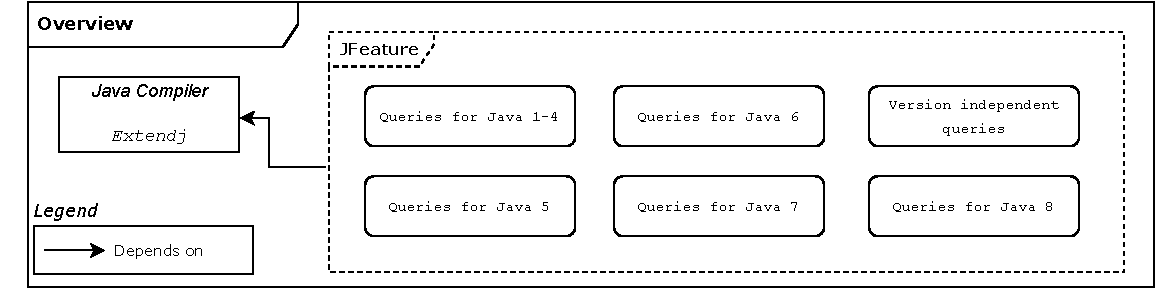
\includegraphics[width=1\textwidth]{kappa/img/JFeature.pdf}
  \caption{\label{fig:JFeature} \textsc{JFeature} architecture.}
\end{figure}

We conduced a case study, applying \textsc{JFeature} to four widely used corpora in the
program analysis area: the \textsc{Da Capo Benchmark suite}, \textsc{Defects4J}~\cite{just2014defects4j}, \textsc{Qualitas Corpus}~\cite{QualitasCorpus:APSEC:2010}, and \textsc{XCorpus}~\cite{dietrich2017xcorpus}.
The results showed that Java 1-5 features were predominant among the corpora,
suggesting that some of the corpora may be less suited for the evaluation of 
tools that address features in Java 7 and 8.
In addition to evaluating corpora, we showed how \textsc{JFeature} could also be used for other
applications such as longitudinal studies of individual Java projects and the creation 
of new corpora. In Paper II, we aslo demonstrate a practical application of how \textsc{JFeature} can 
be extended to capture more complex semantic features by writing queries using the RAGs formalism.


